% This is the Reed College LaTeX thesis template. Most of the work
% for the document class was done by Sam Noble (SN), as well as this
% template. Later comments etc. by Ben Salzberg (BTS). Additional
% restructuring and APA support by Jess Youngberg (JY).
% Your comments and suggestions are more than welcome; please email
% them to cus@reed.edu
%
% See https://www.reed.edu/cis/help/LaTeX/index.html for help. There are a
% great bunch of help pages there, with notes on
% getting started, bibtex, etc. Go there and read it if you're not
% already familiar with LaTeX.
%
% Any line that starts with a percent symbol is a comment.
% They won't show up in the document, and are useful for notes
% to yourself and explaining commands.
% Commenting also removes a line from the document;
% very handy for troubleshooting problems. -BTS

% As far as I know, this follows the requirements laid out in
% the 2002-2003 Senior Handbook. Ask a librarian to check the
% document before binding. -SN

%%
%% Preamble
%%
% \documentclass{<something>} must begin each LaTeX document
\documentclass[12pt,twoside]{reedthesis}
% Packages are extensions to the basic LaTeX functions. Whatever you
% want to typeset, there is probably a package out there for it.
% Chemistry (chemtex), screenplays, you name it.
% Check out CTAN to see: https://www.ctan.org/
%%
\usepackage{graphicx,latexsym}
\usepackage{amsmath}
\usepackage{amssymb,amsthm}
\usepackage{longtable,booktabs,setspace}
\usepackage{chemarr} %% Useful for one reaction arrow, useless if you're not a chem major
\usepackage[hyphens]{url}
% Added by CII
\usepackage{hyperref}
\usepackage{lmodern}
\usepackage{float}
\floatplacement{figure}{H}
% Thanks, @Xyv
\usepackage{calc}
% End of CII addition
\usepackage{rotating}

% Next line commented out by CII
%%% \usepackage{natbib}
% Comment out the natbib line above and uncomment the following two lines to use the new
% biblatex-chicago style, for Chicago A. Also make some changes at the end where the
% bibliography is included.
%\usepackage{biblatex-chicago}
%\bibliography{thesis}


% Added by CII (Thanks, Hadley!)
% Use ref for internal links
\renewcommand{\hyperref}[2][???]{\autoref{#1}}
\def\chapterautorefname{Chapter}
\def\sectionautorefname{Section}
\def\subsectionautorefname{Subsection}
% End of CII addition

% Added by CII
\usepackage{caption}
\captionsetup{width=5in}
% End of CII addition

% \usepackage{times} % other fonts are available like times, bookman, charter, palatino

% Syntax highlighting #22
  \usepackage{color}
  \usepackage{fancyvrb}
  \newcommand{\VerbBar}{|}
  \newcommand{\VERB}{\Verb[commandchars=\\\{\}]}
  \DefineVerbatimEnvironment{Highlighting}{Verbatim}{commandchars=\\\{\}}
  % Add ',fontsize=\small' for more characters per line
  \usepackage{framed}
  \definecolor{shadecolor}{RGB}{248,248,248}
  \newenvironment{Shaded}{\begin{snugshade}}{\end{snugshade}}
  \newcommand{\AlertTok}[1]{\textcolor[rgb]{0.94,0.16,0.16}{#1}}
  \newcommand{\AnnotationTok}[1]{\textcolor[rgb]{0.56,0.35,0.01}{\textbf{\textit{#1}}}}
  \newcommand{\AttributeTok}[1]{\textcolor[rgb]{0.77,0.63,0.00}{#1}}
  \newcommand{\BaseNTok}[1]{\textcolor[rgb]{0.00,0.00,0.81}{#1}}
  \newcommand{\BuiltInTok}[1]{#1}
  \newcommand{\CharTok}[1]{\textcolor[rgb]{0.31,0.60,0.02}{#1}}
  \newcommand{\CommentTok}[1]{\textcolor[rgb]{0.56,0.35,0.01}{\textit{#1}}}
  \newcommand{\CommentVarTok}[1]{\textcolor[rgb]{0.56,0.35,0.01}{\textbf{\textit{#1}}}}
  \newcommand{\ConstantTok}[1]{\textcolor[rgb]{0.00,0.00,0.00}{#1}}
  \newcommand{\ControlFlowTok}[1]{\textcolor[rgb]{0.13,0.29,0.53}{\textbf{#1}}}
  \newcommand{\DataTypeTok}[1]{\textcolor[rgb]{0.13,0.29,0.53}{#1}}
  \newcommand{\DecValTok}[1]{\textcolor[rgb]{0.00,0.00,0.81}{#1}}
  \newcommand{\DocumentationTok}[1]{\textcolor[rgb]{0.56,0.35,0.01}{\textbf{\textit{#1}}}}
  \newcommand{\ErrorTok}[1]{\textcolor[rgb]{0.64,0.00,0.00}{\textbf{#1}}}
  \newcommand{\ExtensionTok}[1]{#1}
  \newcommand{\FloatTok}[1]{\textcolor[rgb]{0.00,0.00,0.81}{#1}}
  \newcommand{\FunctionTok}[1]{\textcolor[rgb]{0.00,0.00,0.00}{#1}}
  \newcommand{\ImportTok}[1]{#1}
  \newcommand{\InformationTok}[1]{\textcolor[rgb]{0.56,0.35,0.01}{\textbf{\textit{#1}}}}
  \newcommand{\KeywordTok}[1]{\textcolor[rgb]{0.13,0.29,0.53}{\textbf{#1}}}
  \newcommand{\NormalTok}[1]{#1}
  \newcommand{\OperatorTok}[1]{\textcolor[rgb]{0.81,0.36,0.00}{\textbf{#1}}}
  \newcommand{\OtherTok}[1]{\textcolor[rgb]{0.56,0.35,0.01}{#1}}
  \newcommand{\PreprocessorTok}[1]{\textcolor[rgb]{0.56,0.35,0.01}{\textit{#1}}}
  \newcommand{\RegionMarkerTok}[1]{#1}
  \newcommand{\SpecialCharTok}[1]{\textcolor[rgb]{0.00,0.00,0.00}{#1}}
  \newcommand{\SpecialStringTok}[1]{\textcolor[rgb]{0.31,0.60,0.02}{#1}}
  \newcommand{\StringTok}[1]{\textcolor[rgb]{0.31,0.60,0.02}{#1}}
  \newcommand{\VariableTok}[1]{\textcolor[rgb]{0.00,0.00,0.00}{#1}}
  \newcommand{\VerbatimStringTok}[1]{\textcolor[rgb]{0.31,0.60,0.02}{#1}}
  \newcommand{\WarningTok}[1]{\textcolor[rgb]{0.56,0.35,0.01}{\textbf{\textit{#1}}}}

% To pass between YAML and LaTeX the dollar signs are added by CII
\title{My Final College Paper}
\author{Ingrid Tallulah Loraine Zoll}
% The month and year that you submit your FINAL draft TO THE LIBRARY (May or December)
\date{May 2022}
\division{Mathematics and Natural Sciences}
\advisor{Aaron Ramirez}
\institution{Reed College}
\degree{Bachelor of Arts}
%If you have two advisors for some reason, you can use the following
% Uncommented out by CII
\altadvisor{Anna Ritz}
% End of CII addition

%%% Remember to use the correct department!
\department{Biology}
% if you're writing a thesis in an interdisciplinary major,
% uncomment the line below and change the text as appropriate.
% check the Senior Handbook if unsure.
%\thedivisionof{The Established Interdisciplinary Committee for}
% if you want the approval page to say "Approved for the Committee",
% uncomment the next line
%\approvedforthe{Committee}

% Added by CII
%%% Copied from knitr
%% maxwidth is the original width if it's less than linewidth
%% otherwise use linewidth (to make sure the graphics do not exceed the margin)
\makeatletter
\def\maxwidth{ %
  \ifdim\Gin@nat@width>\linewidth
    \linewidth
  \else
    \Gin@nat@width
  \fi
}
\makeatother

% From {rticles}
\newlength{\csllabelwidth}
\setlength{\csllabelwidth}{3em}
\newlength{\cslhangindent}
\setlength{\cslhangindent}{1.5em}
% for Pandoc 2.8 to 2.10.1
\newenvironment{cslreferences}%
  {}%
  {\par}
% For Pandoc 2.11+
% As noted by @mirh [2] is needed instead of [3] for 2.12
\newenvironment{CSLReferences}[2] % #1 hanging-ident, #2 entry spacing
 {% don't indent paragraphs
  \setlength{\parindent}{0pt}
  % turn on hanging indent if param 1 is 1
  \ifodd #1 \everypar{\setlength{\hangindent}{\cslhangindent}}\ignorespaces\fi
  % set entry spacing
  \ifnum #2 > 0
  \setlength{\parskip}{#2\baselineskip}
  \fi
 }%
 {}
\usepackage{calc} % for calculating minipage widths
\newcommand{\CSLBlock}[1]{#1\hfill\break}
\newcommand{\CSLLeftMargin}[1]{\parbox[t]{\csllabelwidth}{#1}}
\newcommand{\CSLRightInline}[1]{\parbox[t]{\linewidth - \csllabelwidth}{#1}}
\newcommand{\CSLIndent}[1]{\hspace{\cslhangindent}#1}

\renewcommand{\contentsname}{Table of Contents}
% End of CII addition

\setlength{\parskip}{0pt}

% Added by CII

\providecommand{\tightlist}{%
  \setlength{\itemsep}{0pt}\setlength{\parskip}{0pt}}

\Acknowledgements{
I want to thank a few people.
}

\Dedication{
You can have a dedication here if you wish.
}

\Preface{
This is an example of a thesis setup to use the reed thesis document class
(for LaTeX) and the R bookdown package, in general.
}

\Abstract{
The preface pretty much says it all.

\par

Second paragraph of abstract starts here.
}

	\usepackage{setspace}\onehalfspacing
% End of CII addition
%%
%% End Preamble
%%
%
\begin{document}

% Everything below added by CII
  \maketitle

\frontmatter % this stuff will be roman-numbered
\pagestyle{empty} % this removes page numbers from the frontmatter
  \begin{acknowledgements}
    I want to thank a few people.
  \end{acknowledgements}
  \begin{preface}
    This is an example of a thesis setup to use the reed thesis document class
    (for LaTeX) and the R bookdown package, in general.
  \end{preface}
  \hypersetup{linkcolor=black}
  \setcounter{secnumdepth}{2}
  \setcounter{tocdepth}{2}
  \tableofcontents

  \listoftables

  \listoffigures
  \begin{abstract}
    The preface pretty much says it all.

    \par

    Second paragraph of abstract starts here.
  \end{abstract}
  \begin{dedication}
    You can have a dedication here if you wish.
  \end{dedication}
\mainmatter % here the regular arabic numbering starts
\pagestyle{fancyplain} % turns page numbering back on

\hypertarget{intro}{%
\chapter{Introduction}\label{intro}}

\hypertarget{urban-forests-and-urbanization}{%
\section{Urban Forests and Urbanization}\label{urban-forests-and-urbanization}}

An urban forest is the total population of trees in an urban area. Urban forests are comprised of parks, street trees, landscaped boulevards, green spaces, and any other location where trees can be found in urban spaces. Urban forests are in close proximity to large or dense human populations, have a relatively high diversity of species and forest patch structures as well as both public and private ownership, and their management is often geared toward sustaining tree health and maximizing the potential benefits that trees provide (Robertson \& Mason, 2016). In 2011, urban forests in the United States contained around 74.4 billion trees, which is about a quarter of the total tree population (USDA Forest Service, 2011). The US Census bureau reports that, in 2010, nearly 81\% of Americans lived in urban areas, up from 79\% 10 years earlier . The United Nations predicts that, by 2050, 68\% of the world population will live in urban areas (United Nations \& Affairs, 2018). As urbanization continues, it becomes increasingly important for both those working to manage urban forests and residents of urban areas to understand the dynamics and health of urban forests in order to retain and protect the numerous benefits they provide.

\hypertarget{the-benefits-of-urban-forests}{%
\section{The Benefits of Urban Forests}\label{the-benefits-of-urban-forests}}

Urban forests and urban trees have numerous benefits, which range from environmental to economic. The environmental benefits of urban trees include numerous forms of pollution removal from both water and air. In undeveloped areas, most of the precipitated water is absorbed into the earth. However, due to the high amount of impervious surfaces such as sidewalks, streets, and parking lots in urban areas, rain and snowmelt are unable to soak back into the earth and become stormwater runoff instead. This runoff flows over developed impervious surfaces and picks up trash, yard waste, dirt, and many other potentially harmful chemicals and pollutants. It is then deposited in streams, rivers, wetlands, and other bodies of water that are damaged by polluted runoff. Green infrastructure like urban trees help in reducing the volume and rate of runoff by allowing more precipitation to be soaked into the earth. Research has shown that the presence of street trees also has a positive impact in reducing stormwater runoff volume (US EPA, 2020). A 2021 study conducted in Fond du Lac, Wisconsin, showed that the removal of street trees increased the volume of stormwater runoff by 4\% (Selbig et al., 2021). The study calculated that on a per-tree basis for each square meter of canopy that was removed, 66 liters of rainfall could have been intercepted and stored by the street trees. This results in an annual runoff volume reduction estimated at 6,376 liters per tree.

Urban trees also remove pollutants from the air. Numerous studies have shown that trees can remove many different pollutants (O3, PM10, NO2, SO2, CO) by uptake via leaf stomata. Pollutant particles can also be collected and stored on a tree's surface. Urban trees provide a total annual air pollution removal of 711,000 tons, which is valued at \$3.8 billion (David J. Nowak, Crane, \& Stevens, 2006). Cities with higher levels of tree canopy cover have higher rates of pollution removal by trees, and longer on-leaf growing periods of trees lead to more pollution removal as well. While the removal of air pollution by urban trees results in the improvement of air quality, trees also help mitigate climate change, improve atmospheric conditions and air quality through carbon sequestration.

The increase of atmospheric carbon dioxide from human sources is one of the primary drivers of global climate change. In 2019, U.S. greenhouse gas emissions totaled 6,558 million metric tons of carbon dioxide equivalents. In the same year, the city of Portland's carbon emissions totaled around 55,000 metric tons of carbon dioxide equivalents (City of Portland, 2020). Rural and urban forests, as well as other natural and nature based carbon sinks have been suggested as a method of mitigating greenhouse gas emissions of cities in order to reduce the impacts of global climate change (Lazarus, Chandler, \& Erickson, 2013). These natural carbon sinks capture atmospheric carbon dioxide during photosynthesis and store the carbon as biomass, releasing oxygen back into the atmosphere.

Multiple scholars estimate that urban trees in the United States currently store over 708 million tons of carbon, and capture another 28.2 million tons of carbon per year, which is approximately 0.05\% of annual carbon dioxide emissions in the United States (David J. Nowak \& Crane, 2002; David J. Nowak, Greenfield, Hoehn, \& Lapoint, 2013; Safford, Larry, McPherson, Nowak, \& Westphal, 2013). The current carbon storage of urban trees is valued at more than \$50 billion, with carbon sequestration valued at an additional \$2 billion per year (David J. Nowak et al., 2013). The environmental benefits of urban trees can result in economic advantages under future carbon trading schemas, but there are other unique economic and social benefits that urban trees provide.

Residents of urban areas experience the benefits of urban trees most immediately through the beauty and visual stimulation they provide. Aesthetics alone are a large driver in the plantings of urban trees. Studies have found that trees are one of the main contributors to positive visual aesthetic quality of residential areas, and that large trees contribute more to perceived beauty than smaller trees (Herbert W. Schroeder, 2011; Herbert W. Schroeder \& Cannon, 1987; H. Schroeder \& Cannon, 1983).

The positive impacts of urban trees goes far beyond their visual contributions. Numerous studies have shown that people living near urban forests live longer, experience better mental health, and self-rate their overall health higher than people who do not live near urban forests (James, Banay, Hart, \& Laden, 2015). Residents of two different towns in Germany visited urban forests and green spaces more frequently after the beginning of the COVID-19 pandemic, which contributed significantly to the residents' well-being (Beckmann-Wübbelt et al., 2021). Research into the psychological benefits of urban trees shows that teenage girls who spend more time around trees and other sources of nature and vegetation have higher levels of self-discipline, and children with diagnosed attention deficit disorder show improved focus and ability to learn after spending time outside (Taylor, Kuo, \& Sullivan, 2002; Taylor, Kuo, \& Sullivan, 2001).

Additionally, urban trees provide numerous economic benefits on both a nation wide scale, and an individual scale. Urban tree canopy cover positively impacts residential property values. In Athens, Georgia, landscaping with trees results in a 3.5\%--4.5\% increase in home sale price (Anderson \& Cordell, 1988). In Ramsey and Dakota Counties, Minnesota, researchers found that a 10\% increase in tree cover within 100m of a house increases the average home price by 0.5\% (Sander, Polasky, \& Haight, 2010). Both summer cooling and winter heating demands can be reduced through shading and wind speed reduction by urban trees, which lowers energy costs (David J. Nowak et al., 2010). A 2009 study of 460 single-family homes in Sacramento, California showed that tree cover on the south and west sides of houses reduced summer electricity use by 5.2\%, whereas trees on the north side of a house increased electricity use by 1.5\% (Donovan \& Butry, 2009). A more recent study conducted in the city of Thessaloniki in northern Greece found that the cooling potential of street trees is directly related to the foliage density and the shade provided can lower temperatures up to 5 degrees C, leading to energy savings of up to 54\% (Tsoka, Leduc, \& Rodler, 2021).

\hypertarget{environmental-challenges-for-urban-trees}{%
\section{Environmental Challenges for Urban Trees}\label{environmental-challenges-for-urban-trees}}

Human activities have impacted and altered the Earth's climate and land surface at a fundamental level. These changes have led to the creation of a new geologic epoch, known as the Anthropocene (Huang, Anderegg, \& Asner, 2019). The Anthropocene has seen elevated temperatures and prolonged droughts. These extreme droughts can trigger extensive forest die-off as well as increased tree and shrub mortality rates, which has impacted forests and woodlands on all vegetated continents. Remote sensing research on the impacts of droughts has shown that the impacts of a drought can produce a suppression of forest canopy greenness, which relates to a failing of plant ecophysiological processes and a reduction of chlorophyll. Droughts are predicted to occur more frequently and have higher intensities as we progress through the Anthropocene.

The impacts of climate change and the environmental challenges that all trees will face is even more extreme in urban areas. The multiple economic, environmental and quality of life, health benefits that are provided by urban trees are dependent on tree health. Urban trees are generally more stressed than those in rural areas due to the adverse growing conditions they face. This includes higher temperatures, additional soil compaction, root zone restrictions, and extreme variations in environmental conditions such as wind speed and sunlight level (Flint, 1985; Ward \& Johnson, 2007). Monitoring and tracking tree health over time is an essential component for the ability to model and predict the future changes that will occur. Research into the remote sensing of health indicators of forest die-off has shown that vegetation greenness metrics, such as NDVI, reflect the changes that occur with tree die-off (Breshears et al., 2005; Byer \& Jin, 2017). In order to work towards understanding these changes and how to mitigate the impacts of forest die-off, it is extremely important to understand the current health dynamics of urban forests at a city-wide level, and carefully track changes in urban forest health over time.

\hypertarget{urban-forestry-in-portland-oregon}{%
\section{Urban Forestry in Portland, Oregon}\label{urban-forestry-in-portland-oregon}}

Portland is one of many cities to create tree inventories in the last 25 years, with the goal of better understanding the urban forest. Over a period of 9 years, 2,000 volunteers along with members of Portland's Urban Forestry team inventoried Portland's 245,000 park and street trees (DiSalvo, Fukuda, Ramsey, \& Parks, 2017; Portland Urban Forestry, 2019). In addition to basic physical and environmental variables such as tree height, diameter, and location, volunteers also visually assessed the health condition of each tree, and categorized it as good, fair, poor, or dead. Portland inventoried the 218,602 street trees between 2010 and 2016, and 25,740 park trees between 2017 and 2019. Portland Urban Forestry estimates that Portland's parks contain upwards of 1.2 million trees, but the tree inventory project only inventoried trees in developed portions of parks. Portland Urban Forestry estimates that Portland's street trees produce an estimated \$28.6 million annually in environmental and aesthetic benefits, with a full replacement value of \$753 million (DiSalvo et al., 2017). Portland's inventoried park trees have an estimated worth of \$128 million (Portland Urban Forestry, 2019). While Portland's tree inventories are spectacular resources which help shed light on the urban tree population in Portland and the benefits it can provide, there are limitations to the information available through the inventories.

One drawback of the inventories is that volunteers were only able to inventory trees on public land, which excluded any trees growing in yards or other privately owned areas. Since only developed portions of parks were inventoried, roughly 98\% of Portland's park trees were not inventoried. Additionally, since the inventories were collected over a 9 year period, the collected health assessments for many trees are no longer reliable or representative of present day conditions. They represent data from a range of 9 years and in the 11 years since inventory collection began much has changed.

Measuring urban tree health through field surveys can be extremely time and labor intensive. It requires the collection of detailed data on numerous environmental variables, as well as extensive groundwork to conduct the field surveys. To collect Portland's tree inventories, more than 2,000 volunteers collectively spend upwards of 25,000 hours in the field. Additionally, in order to get a good picture of changes in tree health over time, trees need to be revisited numerous times over the study period. Remote sensing data from satellite imagery can be used to locate and map trees in both urban and rural areas, as well as monitor tree health.

\hypertarget{remote-sensing}{%
\section{Remote Sensing}\label{remote-sensing}}

While the term ``remote sensing'' was first used in the 1960s, the first aerial images were taken in the 1850s from hot air balloons. Later, small cameras were attached to kites and even pigeons to capture aerial images. With the development of airplanes in the early 20th century, images were able to be taken from higher altitudes, providing aerial views of larger surface areas (Moore, 1979). Aerial images taken from planes provided essential military reconnaissance during both World War I and II. The first environmental applications of aerial imagery began in the 1930s, when the Agriculture Department began to use aerial photography to map and catalog farmland in the United States. Soon after, aerial imagery became a tool for conservation and land planning purposes. Capturing aerial images from planes was the primary method of capturing images of the earth's surface until the early 1960s. Since the first satellite was launched in 1957, the technical capabilities of satellites has greatly increased, along with the types and applications of satellite-collected data (Khorram, 2012).

Within the field of forestry and ecology, remote sensing has numerous applications, from measuring the cover and structure of vegetation, to examining biodiversity and soil characteristics of specific areas. Additionally, remote sensing measurements can be used to calculate and monitor changes in forest density, which is critical for determining the fuel load and forest health in regards to fire risk. One of the most commonly used remote sensing metrics used to measure forest health is the Normalized Difference Vegetation Index (NDVI), which is calculated from the red and near infrared (NIR) bands from remote sensing imagery. Studies have shown that NDVI is highly correlated with chlorophyll content. Specifically, NDVI has a near-linear relationship to the chlorophyll content of soybean crops (Myneni, Hall, Sellers, \& Marshak, 1995; Tucker, 1979). Especially when the goal is monitoring tree health changes over time, remote sensing data eliminates the need for repeated sampling over long time periods, since satellite images are taken at regular intervals as the satellites continually orbit the earth. With the availability and accuracy of aerial imagery increasing as these technologies continue to advance, remote sensing is becoming an important and effective method for mapping, monitoring, and analyzing tree health on an individual tree scale (Xiao \& McPherson, 2005).

\hypertarget{previous-work}{%
\section{Previous work}\label{previous-work}}

Xiao \& McPherson (2005) used multispectral remote sensing data paired with field collected tree health data with the goal of mapping tree health on the University of California Davis campus. Field data on 81 campus trees was collected in the summer of 2004, and the health of the trees was classified as ``healthy'' or ``unhealthy.'' Additionally, a second dataset of 1,186 trees was collected which included randomly selected trees to check the accuracy of the resulting tree health mapping. With high resolution multispectral remote sensing data collected in the summers of 2003 and 2004, NDVI was calculated and used to classify each pixel as vegetation or non-vegetation. The pixels representing trees and shrubs were manually selected and extracted, resulting in NDVI data just for trees and shrubs. The remaining data was split into 5 separate layers based on physiognomic tree type (broadleaf deciduous, broadleaf evergreen, conifer, palm, and mixed). Tree health was evaluated at both a pixel scale, and a tree scale, with the pixels or trees being mapped as either healthy or unhealthy. A tree was labeled as unhealthy if 30\% or more of the pixels within the manually delineated tree crown were mapped as unhealthy, and if the average NDVI of the pixels were less than the NDVI threshold for healthy trees. The accuracy of the tree health assessment was checked against the validation dataset of 1,186 trees. The field health assessment agreed with the remotely sensed health classification for 88\% of the trees.

Fang, McNeil, Warner, Dahle, \& Eutsler (2020) used a similar approach to evaluate the health of street trees in Washington D.C. using multispectral remote sensing data and D.C.'s street tree inventory. The tree inventory contained 18,434 trees, each with a tree health classification of excellent, good, fair, poor, or dead. The researchers purchased remote sensing images for June 11, July 30, and August 30, 2017, to compare the sensitivity of tree health at different points in the trees' on-leaf period. To extract pixels belonging to tree crowns, a radial buffer based on tree crown diameter was used, and pixels with low NDVI values were masked. This paper tested 5 different vegetation indices (VIs), which included three different variations of NDVI. The different VIs were calculated for each pixel and averaged for each tree. They found that the VI values of trees in good, fair, and poor health conditions were highly statistically different, and traditional NDVI was the most sensitive VI for detecting tree health conditions. Additionally, it was determined that remote sensing imagery taken in the middle of the on-leaf period had the best potential to assess the health condition of trees.

These two studies form the basis of the approach and methods for this thesis, but there are two main places where I believe I can add new insights and improve methodology. First, a frustrating drawback of both Fang et al. (2020) and Xiao \& McPherson (2005) is that a true replication of their process is inaccessible due to the sources of their data. Xiao \& McPherson (2005) used multispectral data that was specially collected just for the UC Davis campus, and Fang et al. (2020) purchased the high resolution multispectral data that was used in their study. Second, there is little consistency in the methods used to select image pixels for NDVI evaluation. Xiao \& McPherson (2005) manually detected and delineated tree crowns for health assessment, and any trees with overlapping crowns were removed from the analysis. Manual crown delineation is extremely time intensive and is an unrealistic method for large sample sizes. In Fang et al. (2020), a standardized radius based on the average DBH of all trees was used to select the tree crown area. However, this method will only use the center pixels of large trees eliminating the edges, and it is unclear how overlapping tree crowns were dealt with. The impact of these different methods on health analysis is unknown.

\hypertarget{this-thesis}{%
\section{This Thesis}\label{this-thesis}}

Based on the assumptions that tree health can be approximated using satellite spectral data, specifically NDVI, this thesis aims to replicate the process of Fang et al. (2020) and Xiao \& McPherson (2005). Additionally, I will investigate the questions of the impact of species differentiation when using NDVI to calculate tree health, and if different methods of tree crown delineation impact the health rating outcome. Based on these questions, I predict that differentiating health rating predictions by tree species will improve the accuracy of the model, and differentiating by tree type (coniferous evergreen vs broadleaf deciduous trees) will also improve the accuracy, but less than species. Additionally, I predict that using more in-depth tree crown delineation approaches will allow for more trees to be analyzed, and will also improve the accuracy of the health rating.

Finally, this thesis only uses data sources, tools, and processes that are either publicly accessible or free, in order to keep this type of research accessible to all.

\hypertarget{math-sci}{%
\chapter{Mathematics and Science}\label{math-sci}}

\hypertarget{math}{%
\section{Math}\label{math}}

\TeX~is the best way to typeset mathematics. Donald Knuth designed \TeX~when he got frustrated at how long it was taking the typesetters to finish his book, which contained a lot of mathematics. One nice feature of \emph{R Markdown} is its ability to read LaTeX code directly.

If you are doing a thesis that will involve lots of math, you will want to read the following section which has been commented out. If you're not going to use math, skip over or delete this next commented section.

\hypertarget{chemistry-101-symbols}{%
\section{Chemistry 101: Symbols}\label{chemistry-101-symbols}}

Chemical formulas will look best if they are not italicized. Get around math mode's automatic italicizing in LaTeX by using the argument \texttt{\$\textbackslash{}mathrm\{formula\ here\}\$}, with your formula inside the curly brackets. (Notice the use of the backticks here which enclose text that acts as code.)

So, \(\mathrm{Fe_2^{2+}Cr_2O_4}\) is written \texttt{\$\textbackslash{}mathrm\{Fe\_2\^{}\{2+\}Cr\_2O\_4\}\$}.

\noindent Exponent or Superscript: \(\mathrm{O^-}\)

\noindent Subscript: \(\mathrm{CH_4}\)

To stack numbers or letters as in \(\mathrm{Fe_2^{2+}}\), the subscript is defined first, and then the superscript is defined.

\noindent Bullet: CuCl \(\bullet\) \(\mathrm{7H_{2}O}\)

\noindent Delta: \(\Delta\)

\noindent Reaction Arrows: \(\longrightarrow\) or \(\xrightarrow{solution}\)

\noindent Resonance Arrows: \(\leftrightarrow\)

\noindent Reversible Reaction Arrows: \(\rightleftharpoons\)

\hypertarget{typesetting-reactions}{%
\subsection{Typesetting reactions}\label{typesetting-reactions}}

You may wish to put your reaction in an equation environment, which means that LaTeX will place the reaction where it fits and will number the equations for you.
\begin{equation}
  \mathrm{C_6H_{12}O_6  + 6O_2} \longrightarrow \mathrm{6CO_2 + 6H_2O}
  \label{eq:reaction}
\end{equation}
We can reference this combustion of glucose reaction via Equation \eqref{eq:reaction}.

\hypertarget{other-examples-of-reactions}{%
\subsection{Other examples of reactions}\label{other-examples-of-reactions}}

\(\mathrm{NH_4Cl_{(s)}}\) \(\rightleftharpoons\) \(\mathrm{NH_{3(g)}+HCl_{(g)}}\)

\noindent \(\mathrm{MeCH_2Br + Mg}\) \(\xrightarrow[below]{above}\) \(\mathrm{MeCH_2\bullet Mg \bullet Br}\)

\hypertarget{physics}{%
\section{Physics}\label{physics}}

Many of the symbols you will need can be found on the math page \url{https://web.reed.edu/cis/help/latex/math.html} and the Comprehensive LaTeX Symbol Guide (\url{https://mirror.utexas.edu/ctan/info/symbols/comprehensive/symbols-letter.pdf}).

\hypertarget{biology}{%
\section{Biology}\label{biology}}

You will probably find the resources at \url{https://www.lecb.ncifcrf.gov/~toms/latex.html} helpful, particularly the links to bsts for various journals. You may also be interested in TeXShade for nucleotide typesetting (\url{https://homepages.uni-tuebingen.de/beitz/txe.html}). Be sure to read the proceeding chapter on graphics and tables.

\hypertarget{ref-labels}{%
\chapter{Graphics, References, and Labels}\label{ref-labels}}

\hypertarget{figures}{%
\section{Figures}\label{figures}}

If your thesis has a lot of figures, \emph{R Markdown} might behave better for you than that other word processor. One perk is that it will automatically number the figures accordingly in each chapter. You'll also be able to create a label for each figure, add a caption, and then reference the figure in a way similar to what we saw with tables earlier. If you label your figures, you can move the figures around and \emph{R Markdown} will automatically adjust the numbering for you. No need for you to remember! So that you don't have to get too far into LaTeX to do this, a couple \textbf{R} functions have been created for you to assist. You'll see their use below.

In the \textbf{R} chunk below, we will load in a picture stored as \texttt{reed.jpg} in our main directory. We then give it the caption of ``Reed logo'', the label of ``reedlogo'', and specify that this is a figure. Make note of the different \textbf{R} chunk options that are given in the R Markdown file (not shown in the knitted document).
\begin{Shaded}
\begin{Highlighting}[]
\FunctionTok{include\_graphics}\NormalTok{(}\AttributeTok{path =} \StringTok{"figure/reed.jpg"}\NormalTok{)}
\end{Highlighting}
\end{Shaded}
\begin{figure}

{\centering 
\includegraphics[width=0.2\linewidth]{figure/reed} 

}

\caption{Reed logo}\label{fig:reedlogo}
\end{figure}
Here is a reference to the Reed logo: Figure \ref{fig:reedlogo}. Note the use of the \texttt{fig:} code here. By naming the \textbf{R} chunk that contains the figure, we can then reference that figure later as done in the first sentence here. We can also specify the caption for the figure via the R chunk option \texttt{fig.cap}.

\clearpage

Below we will investigate how to save the output of an \textbf{R} plot and label it in a way similar to that done above. Recall the \texttt{flights} dataset from Chapter \ref{rmd-basics}. (Note that we've shown a different way to reference a section or chapter here.) We will next explore a bar graph with the mean flight departure delays by airline from Portland for 2014.
\begin{Shaded}
\begin{Highlighting}[]
\NormalTok{mean\_delay\_by\_carrier }\OtherTok{\textless{}{-}}\NormalTok{ flights }\SpecialCharTok{\%\textgreater{}\%}
  \FunctionTok{group\_by}\NormalTok{(carrier) }\SpecialCharTok{\%\textgreater{}\%}
  \FunctionTok{summarize}\NormalTok{(}\AttributeTok{mean\_dep\_delay =} \FunctionTok{mean}\NormalTok{(dep\_delay))}
\FunctionTok{ggplot}\NormalTok{(mean\_delay\_by\_carrier, }\FunctionTok{aes}\NormalTok{(}\AttributeTok{x =}\NormalTok{ carrier, }\AttributeTok{y =}\NormalTok{ mean\_dep\_delay)) }\SpecialCharTok{+}
  \FunctionTok{geom\_bar}\NormalTok{(}\AttributeTok{position =} \StringTok{"identity"}\NormalTok{, }\AttributeTok{stat =} \StringTok{"identity"}\NormalTok{, }\AttributeTok{fill =} \StringTok{"red"}\NormalTok{)}
\end{Highlighting}
\end{Shaded}
\begin{figure}
\centering
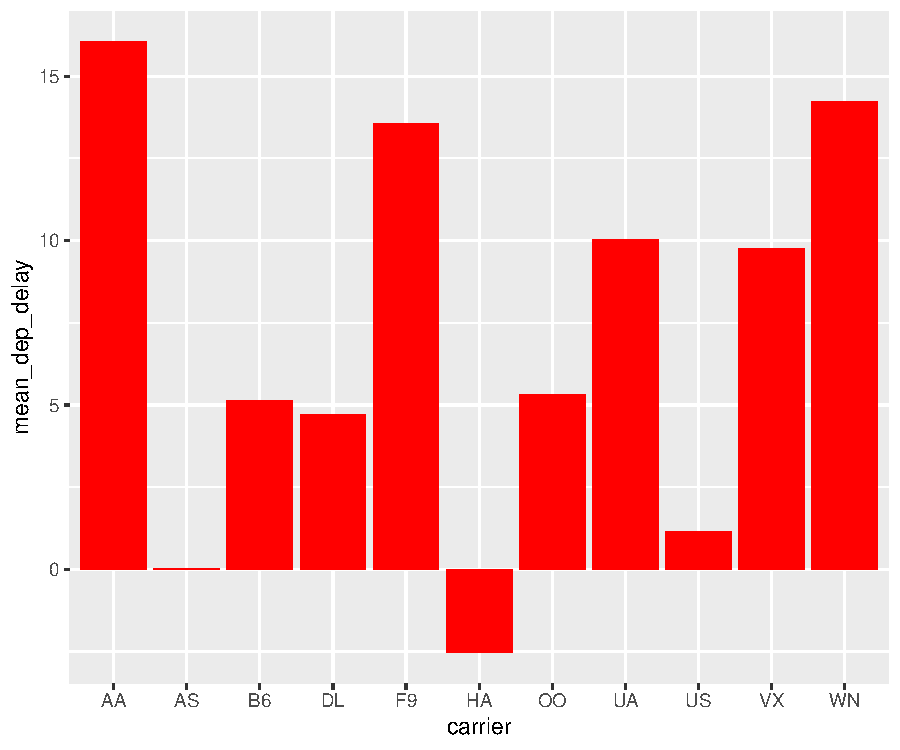
\includegraphics{thesis_files/figure-latex/delaysboxplot-1.pdf}
\caption{\label{fig:delaysboxplot}Mean Delays by Airline}
\end{figure}
Here is a reference to this image: Figure \ref{fig:delaysboxplot}.

A table linking these carrier codes to airline names is available at \url{https://github.com/ismayc/pnwflights14/blob/master/data/airlines.csv}.

\clearpage

Next, we will explore the use of the \texttt{out.extra} chunk option, which can be used to shrink or expand an image loaded from a file by specifying \texttt{"scale=\ "}. Here we use the mathematical graph stored in the ``subdivision.pdf'' file.
\begin{figure}
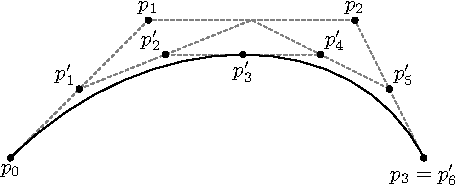
\includegraphics[scale=0.75]{figure/subdivision} \caption{Subdiv. graph}\label{fig:subd}
\end{figure}
Here is a reference to this image: Figure \ref{fig:subd}. Note that \texttt{echo=FALSE} is specified so that the \textbf{R} code is hidden in the document.

\textbf{More Figure Stuff}

Lastly, we will explore how to rotate and enlarge figures using the \texttt{out.extra} chunk option. (Currently this only works in the PDF version of the book.)
\begin{figure}
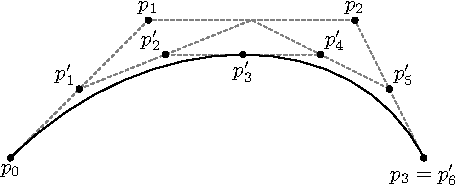
\includegraphics[angle=180, scale=1.1]{figure/subdivision} \caption{A Larger Figure, Flipped Upside Down}\label{fig:subd2}
\end{figure}
As another example, here is a reference: Figure \ref{fig:subd2}.

\hypertarget{footnotes-and-endnotes}{%
\section{Footnotes and Endnotes}\label{footnotes-and-endnotes}}

You might want to footnote something. \footnote{footnote text} The footnote will be in a smaller font and placed appropriately. Endnotes work in much the same way. More information can be found about both on the CUS site or feel free to reach out to \href{mailto:data@reed.edu}{\nolinkurl{data@reed.edu}}.

\hypertarget{bibliographies}{%
\section{Bibliographies}\label{bibliographies}}

Of course you will need to cite things, and you will probably accumulate an armful of sources. There are a variety of tools available for creating a bibliography database (stored with the .bib extension). In addition to BibTeX suggested below, you may want to consider using the free and easy-to-use tool called Zotero. The Reed librarians have created Zotero documentation at \url{https://libguides.reed.edu/citation/zotero}. In addition, a tutorial is available from Middlebury College at \url{https://sites.middlebury.edu/zoteromiddlebury/}.

\emph{R Markdown} uses \emph{pandoc} (\url{https://pandoc.org/}) to build its bibliographies. One nice caveat of this is that you won't have to do a second compile to load in references as standard LaTeX requires. To cite references in your thesis (after creating your bibliography database), place the reference name inside square brackets and precede it by the ``at'' symbol. For example, here's a reference to a book about worrying: (\textbf{Molina1994?}). This \texttt{Molina1994} entry appears in a file called \texttt{thesis.bib} in the \texttt{bib} folder. This bibliography database file was created by a program called BibTeX. You can call this file something else if you like (look at the YAML header in the main .Rmd file) and, by default, is to placed in the \texttt{bib} folder.

For more information about BibTeX and bibliographies, see our CUS site (\url{https://web.reed.edu/cis/help/latex/index.html})\footnote{(\textbf{reedweb2007?})}. There are three pages on this topic: \emph{bibtex} (which talks about using BibTeX, at \url{https://web.reed.edu/cis/help/latex/bibtex.html}), \emph{bibtexstyles} (about how to find and use the bibliography style that best suits your needs, at \url{https://web.reed.edu/cis/help/latex/bibtexstyles.html}) and \emph{bibman} (which covers how to make and maintain a bibliography by hand, without BibTeX, at \url{https://web.reed.edu/cis/help/latex/bibman.html}). The last page will not be useful unless you have only a few sources.

If you look at the YAML header at the top of the main .Rmd file you can see that we can specify the style of the bibliography by referencing the appropriate csl file. You can download a variety of different style files at \url{https://www.zotero.org/styles}. Make sure to download the file into the csl folder.

\vfill

\textbf{Tips for Bibliographies}
\begin{itemize}
\tightlist
\item
  Like with thesis formatting, the sooner you start compiling your bibliography for something as large as thesis, the better. Typing in source after source is mind-numbing enough; do you really want to do it for hours on end in late April? Think of it as procrastination.
\item
  The cite key (a citation's label) needs to be unique from the other entries.
\item
  When you have more than one author or editor, you need to separate each author's name by the word ``and'' e.g.~\texttt{Author\ =\ \{Noble,\ Sam\ and\ Youngberg,\ Jessica\},}.
\item
  Bibliographies made using BibTeX (whether manually or using a manager) accept LaTeX markup, so you can italicize and add symbols as necessary.
\item
  To force capitalization in an article title or where all lowercase is generally used, bracket the capital letter in curly braces.
\item
  You can add a Reed Thesis citation\footnote{(\textbf{noble2002?})} option. The best way to do this is to use the phdthesis type of citation, and use the optional ``type'' field to enter ``Reed thesis'' or ``Undergraduate thesis.''
\end{itemize}
\hypertarget{anything-else}{%
\section{Anything else?}\label{anything-else}}

If you'd like to see examples of other things in this template, please contact the Data @ Reed team (email \href{mailto:data@reed.edu}{\nolinkurl{data@reed.edu}}) with your suggestions. We love to see people using \emph{R Markdown} for their theses, and are happy to help.

\hypertarget{conclusion}{%
\chapter*{Conclusion}\label{conclusion}}
\addcontentsline{toc}{chapter}{Conclusion}

If we don't want Conclusion to have a chapter number next to it, we can add the \texttt{\{-\}} attribute.

\textbf{More info}

And here's some other random info: the first paragraph after a chapter title or section head \emph{shouldn't be} indented, because indents are to tell the reader that you're starting a new paragraph. Since that's obvious after a chapter or section title, proper typesetting doesn't add an indent there.

\appendix

\hypertarget{the-first-appendix}{%
\chapter{The First Appendix}\label{the-first-appendix}}

This first appendix includes all of the R chunks of code that were hidden throughout the document (using the \texttt{include\ =\ FALSE} chunk tag) to help with readibility and/or setup.

\textbf{In the main Rmd file}
\begin{Shaded}
\begin{Highlighting}[]
\CommentTok{\# This chunk ensures that the thesisdown package is}
\CommentTok{\# installed and loaded. This thesisdown package includes}
\CommentTok{\# the template files for the thesis.}
\ControlFlowTok{if}\NormalTok{ (}\SpecialCharTok{!}\FunctionTok{require}\NormalTok{(remotes)) \{}
  \ControlFlowTok{if}\NormalTok{ (params}\SpecialCharTok{$}\StringTok{\textasciigrave{}}\AttributeTok{Install needed packages for \{thesisdown\}}\StringTok{\textasciigrave{}}\NormalTok{) \{}
    \FunctionTok{install.packages}\NormalTok{(}\StringTok{"remotes"}\NormalTok{, }\AttributeTok{repos =} \StringTok{"https://cran.rstudio.com"}\NormalTok{)}
\NormalTok{  \} }\ControlFlowTok{else}\NormalTok{ \{}
    \FunctionTok{stop}\NormalTok{(}
      \FunctionTok{paste}\NormalTok{(}\StringTok{\textquotesingle{}You need to run install.packages("remotes")",}
\StringTok{            "first in the Console.\textquotesingle{}}\NormalTok{)}
\NormalTok{    )}
\NormalTok{  \}}
\NormalTok{\}}
\ControlFlowTok{if}\NormalTok{ (}\SpecialCharTok{!}\FunctionTok{require}\NormalTok{(thesisdown)) \{}
  \ControlFlowTok{if}\NormalTok{ (params}\SpecialCharTok{$}\StringTok{\textasciigrave{}}\AttributeTok{Install needed packages for \{thesisdown\}}\StringTok{\textasciigrave{}}\NormalTok{) \{}
\NormalTok{    remotes}\SpecialCharTok{::}\FunctionTok{install\_github}\NormalTok{(}\StringTok{"ismayc/thesisdown"}\NormalTok{)}
\NormalTok{  \} }\ControlFlowTok{else}\NormalTok{ \{}
    \FunctionTok{stop}\NormalTok{(}
      \FunctionTok{paste}\NormalTok{(}
        \StringTok{"You need to run"}\NormalTok{,}
        \StringTok{\textquotesingle{}remotes::install\_github("ismayc/thesisdown")\textquotesingle{}}\NormalTok{,}
        \StringTok{"first in the Console."}
\NormalTok{      )}
\NormalTok{    )}
\NormalTok{  \}}
\NormalTok{\}}
\FunctionTok{library}\NormalTok{(thesisdown)}
\CommentTok{\# Set how wide the R output will go}
\FunctionTok{options}\NormalTok{(}\AttributeTok{width =} \DecValTok{70}\NormalTok{)}
\end{Highlighting}
\end{Shaded}
\textbf{In Chapter \ref{ref-labels}:}
\begin{Shaded}
\begin{Highlighting}[]
\CommentTok{\# This chunk ensures that the thesisdown package is}
\CommentTok{\# installed and loaded. This thesisdown package includes}
\CommentTok{\# the template files for the thesis and also two functions}
\CommentTok{\# used for labeling and referencing}
\ControlFlowTok{if}\NormalTok{ (}\SpecialCharTok{!}\FunctionTok{require}\NormalTok{(remotes)) \{}
  \ControlFlowTok{if}\NormalTok{ (params}\SpecialCharTok{$}\StringTok{\textasciigrave{}}\AttributeTok{Install needed packages for \{thesisdown\}}\StringTok{\textasciigrave{}}\NormalTok{) \{}
    \FunctionTok{install.packages}\NormalTok{(}\StringTok{"remotes"}\NormalTok{, }\AttributeTok{repos =} \StringTok{"https://cran.rstudio.com"}\NormalTok{)}
\NormalTok{  \} }\ControlFlowTok{else}\NormalTok{ \{}
    \FunctionTok{stop}\NormalTok{(}
      \FunctionTok{paste}\NormalTok{(}
        \StringTok{\textquotesingle{}You need to run install.packages("remotes")\textquotesingle{}}\NormalTok{,}
        \StringTok{"first in the Console."}
\NormalTok{      )}
\NormalTok{    )}
\NormalTok{  \}}
\NormalTok{\}}
\ControlFlowTok{if}\NormalTok{ (}\SpecialCharTok{!}\FunctionTok{require}\NormalTok{(dplyr)) \{}
  \ControlFlowTok{if}\NormalTok{ (params}\SpecialCharTok{$}\StringTok{\textasciigrave{}}\AttributeTok{Install needed packages for \{thesisdown\}}\StringTok{\textasciigrave{}}\NormalTok{) \{}
    \FunctionTok{install.packages}\NormalTok{(}\StringTok{"dplyr"}\NormalTok{, }\AttributeTok{repos =} \StringTok{"https://cran.rstudio.com"}\NormalTok{)}
\NormalTok{  \} }\ControlFlowTok{else}\NormalTok{ \{}
    \FunctionTok{stop}\NormalTok{(}
      \FunctionTok{paste}\NormalTok{(}
        \StringTok{\textquotesingle{}You need to run install.packages("dplyr")\textquotesingle{}}\NormalTok{,}
        \StringTok{"first in the Console."}
\NormalTok{      )}
\NormalTok{    )}
\NormalTok{  \}}
\NormalTok{\}}
\ControlFlowTok{if}\NormalTok{ (}\SpecialCharTok{!}\FunctionTok{require}\NormalTok{(ggplot2)) \{}
  \ControlFlowTok{if}\NormalTok{ (params}\SpecialCharTok{$}\StringTok{\textasciigrave{}}\AttributeTok{Install needed packages for \{thesisdown\}}\StringTok{\textasciigrave{}}\NormalTok{) \{}
    \FunctionTok{install.packages}\NormalTok{(}\StringTok{"ggplot2"}\NormalTok{, }\AttributeTok{repos =} \StringTok{"https://cran.rstudio.com"}\NormalTok{)}
\NormalTok{  \} }\ControlFlowTok{else}\NormalTok{ \{}
    \FunctionTok{stop}\NormalTok{(}
      \FunctionTok{paste}\NormalTok{(}
        \StringTok{\textquotesingle{}You need to run install.packages("ggplot2")\textquotesingle{}}\NormalTok{,}
        \StringTok{"first in the Console."}
\NormalTok{      )}
\NormalTok{    )}
\NormalTok{  \}}
\NormalTok{\}}
\ControlFlowTok{if}\NormalTok{ (}\SpecialCharTok{!}\FunctionTok{require}\NormalTok{(bookdown)) \{}
  \ControlFlowTok{if}\NormalTok{ (params}\SpecialCharTok{$}\StringTok{\textasciigrave{}}\AttributeTok{Install needed packages for \{thesisdown\}}\StringTok{\textasciigrave{}}\NormalTok{) \{}
    \FunctionTok{install.packages}\NormalTok{(}\StringTok{"bookdown"}\NormalTok{, }\AttributeTok{repos =} \StringTok{"https://cran.rstudio.com"}\NormalTok{)}
\NormalTok{  \} }\ControlFlowTok{else}\NormalTok{ \{}
    \FunctionTok{stop}\NormalTok{(}
      \FunctionTok{paste}\NormalTok{(}
        \StringTok{\textquotesingle{}You need to run install.packages("bookdown")\textquotesingle{}}\NormalTok{,}
        \StringTok{"first in the Console."}
\NormalTok{      )}
\NormalTok{    )}
\NormalTok{  \}}
\NormalTok{\}}
\ControlFlowTok{if}\NormalTok{ (}\SpecialCharTok{!}\FunctionTok{require}\NormalTok{(thesisdown)) \{}
  \ControlFlowTok{if}\NormalTok{ (params}\SpecialCharTok{$}\StringTok{\textasciigrave{}}\AttributeTok{Install needed packages for \{thesisdown\}}\StringTok{\textasciigrave{}}\NormalTok{) \{}
\NormalTok{    remotes}\SpecialCharTok{::}\FunctionTok{install\_github}\NormalTok{(}\StringTok{"ismayc/thesisdown"}\NormalTok{)}
\NormalTok{  \} }\ControlFlowTok{else}\NormalTok{ \{}
    \FunctionTok{stop}\NormalTok{(}
      \FunctionTok{paste}\NormalTok{(}
        \StringTok{"You need to run"}\NormalTok{,}
        \StringTok{\textquotesingle{}remotes::install\_github("ismayc/thesisdown")\textquotesingle{}}\NormalTok{,}
        \StringTok{"first in the Console."}
\NormalTok{      )}
\NormalTok{    )}
\NormalTok{  \}}
\NormalTok{\}}
\FunctionTok{library}\NormalTok{(thesisdown)}
\FunctionTok{library}\NormalTok{(dplyr)}
\FunctionTok{library}\NormalTok{(ggplot2)}
\FunctionTok{library}\NormalTok{(knitr)}
\NormalTok{flights }\OtherTok{\textless{}{-}} \FunctionTok{read.csv}\NormalTok{(}\StringTok{"data/flights.csv"}\NormalTok{, }\AttributeTok{stringsAsFactors =} \ConstantTok{FALSE}\NormalTok{)}
\end{Highlighting}
\end{Shaded}
\hypertarget{the-second-appendix-for-fun}{%
\chapter{The Second Appendix, for Fun}\label{the-second-appendix-for-fun}}

\backmatter

\hypertarget{references}{%
\chapter*{References}\label{references}}
\addcontentsline{toc}{chapter}{References}

\markboth{References}{References}

\noindent

\setlength{\parindent}{-0.20in}

\hypertarget{refs}{}
\begin{CSLReferences}{1}{0}
\leavevmode\vadjust pre{\hypertarget{ref-anderson1988}{}}%
Anderson, L. M., \& Cordell, H. K. (1988). Influence of trees on residential property values in Athens, Georgia (U.S.A.): A survey based on actual sales prices. \emph{Landscape and Urban Planning}, \emph{15}(1), 153--164. http://doi.org/\href{https://doi.org/10.1016/0169-2046(88)90023-0}{10.1016/0169-2046(88)90023-0}

\leavevmode\vadjust pre{\hypertarget{ref-beckmann-wuxfcbbelt2021}{}}%
Beckmann-Wübbelt, A., Fricke, A., Sebesvari, Z., Yakouchenkova, I. A., Fröhlich, K., \& Saha, S. (2021). High public appreciation for the cultural ecosystem services of urban and peri{\nobreakdash-}urban forests during the COVID-19 pandemic. \emph{Sustainable Cities and Society}, \emph{74}, 103240. http://doi.org/\href{https://doi.org/10.1016/j.scs.2021.103240}{10.1016/j.scs.2021.103240}

\leavevmode\vadjust pre{\hypertarget{ref-breshears2005}{}}%
Breshears, D. D., Cobb, N. S., Rich, P. M., Price, K. P., Allen, C. D., Balice, R. G., \ldots{} Meyer, C. W. (2005). Regional vegetation die-off in response to global-change-type drought. \emph{Proceedings of the National Academy of Sciences}, \emph{102}(42), 15144--15148. http://doi.org/\href{https://doi.org/10.1073/pnas.0505734102}{10.1073/pnas.0505734102}

\leavevmode\vadjust pre{\hypertarget{ref-byer2017}{}}%
Byer, S., \& Jin, Y. (2017). Detecting Drought-Induced Tree Mortality in Sierra Nevada Forests with Time Series of Satellite Data. \emph{Remote Sensing}, \emph{9}(9), 929. http://doi.org/\href{https://doi.org/10.3390/rs9090929}{10.3390/rs9090929}

\leavevmode\vadjust pre{\hypertarget{ref-cityofportland}{}}%
City of Portland. (2020). Carbon emissions. Retrieved from \url{https://www.portland.gov/bps/scg/scg-dashboard/carbon-emissions}

\leavevmode\vadjust pre{\hypertarget{ref-disalvo2017}{}}%
DiSalvo, A., Fukuda, J., Ramsey, J., \& Parks, P. (2017). \emph{Street Tree Inventory Report: City of Portland} (p. 48).

\leavevmode\vadjust pre{\hypertarget{ref-donovan2009}{}}%
Donovan, G., \& Butry, D. (2009). The value of shade: Estimating the effect of urban trees on summertime electricity use. \emph{Energy and Buildings}, \emph{41}, 662--668. http://doi.org/\href{https://doi.org/10.1016/j.enbuild.2009.01.002}{10.1016/j.enbuild.2009.01.002}

\leavevmode\vadjust pre{\hypertarget{ref-fang2020}{}}%
Fang, F., McNeil, B., Warner, T., Dahle, G., \& Eutsler, E. (2020). Street tree health from space? An evaluation using WorldView-3 data and the Washington D.C. Street Tree Spatial Database. \emph{Urban forestry \& urban greening}, \emph{49}, 126634--. http://doi.org/\href{https://doi.org/10.1016/j.ufug.2020.126634}{10.1016/j.ufug.2020.126634}

\leavevmode\vadjust pre{\hypertarget{ref-flint1985}{}}%
Flint, H. L. (1985). Plants showing tolerance of urban stress. \emph{Journal of Environmental Horticulture}, \emph{3}(2), 85--89. http://doi.org/\href{https://doi.org/10.24266/0738-2898-3.2.85}{10.24266/0738-2898-3.2.85}

\leavevmode\vadjust pre{\hypertarget{ref-huang2019}{}}%
Huang, C., Anderegg, W. R. L., \& Asner, G. P. (2019). Remote sensing of forest die-off in the Anthropocene: From plant ecophysiology to canopy structure. \emph{Remote Sensing of Environment}, \emph{231}, 111233. http://doi.org/\href{https://doi.org/10.1016/j.rse.2019.111233}{10.1016/j.rse.2019.111233}

\leavevmode\vadjust pre{\hypertarget{ref-james2015}{}}%
James, P., Banay, R. F., Hart, J. E., \& Laden, F. (2015). A Review of the Health Benefits of Greenness. \emph{Current Epidemiology Reports}, \emph{2}(2), 131--142. http://doi.org/\href{https://doi.org/10.1007/s40471-015-0043-7}{10.1007/s40471-015-0043-7}

\leavevmode\vadjust pre{\hypertarget{ref-khorram2012}{}}%
Khorram, S. (2012). \emph{Remote Sensing} (1st ed. 2012.). New York, NY: Springer New York : Imprint: Springer.

\leavevmode\vadjust pre{\hypertarget{ref-lazarus2013}{}}%
Lazarus, M., Chandler, C., \& Erickson, P. (2013). A core framework and scenario for deep GHG reductions at the city scale. \emph{Energy Policy}, \emph{57}, 563--574. http://doi.org/\href{https://doi.org/10.1016/j.enpol.2013.02.031}{10.1016/j.enpol.2013.02.031}

\leavevmode\vadjust pre{\hypertarget{ref-moore1979}{}}%
Moore, G. K. (1979). What is a picture worth? A history of remote sensing / quelle est la valeur d'une image? Un tour d'horizon de télédétection. \emph{Hydrological Sciences Bulletin}, \emph{24}(4), 477--485. http://doi.org/\href{https://doi.org/10.1080/02626667909491887}{10.1080/02626667909491887}

\leavevmode\vadjust pre{\hypertarget{ref-myneni1995}{}}%
Myneni, R., Hall, F., Sellers, P., \& Marshak, A. (1995). The interpretation of spectral vegetation indexes. \emph{IEEE Transactions on Geoscience and Remote Sensing}. http://doi.org/\href{https://doi.org/10.1109/36.377948}{10.1109/36.377948}

\leavevmode\vadjust pre{\hypertarget{ref-nowak2002}{}}%
Nowak, David J., \& Crane, D. E. (2002). Carbon storage and sequestration by urban trees in the USA. \emph{Environmental Pollution}, \emph{116}(3), 381--389. http://doi.org/\href{https://doi.org/10.1016/S0269-7491(01)00214-7}{10.1016/S0269-7491(01)00214-7}

\leavevmode\vadjust pre{\hypertarget{ref-nowak2006}{}}%
Nowak, David J., Crane, D. E., \& Stevens, J. C. (2006). Air pollution removal by urban trees and shrubs in the United States. \emph{Urban Forestry \& Urban Greening}, \emph{4}(3), 115--123. http://doi.org/\href{https://doi.org/10.1016/j.ufug.2006.01.007}{10.1016/j.ufug.2006.01.007}

\leavevmode\vadjust pre{\hypertarget{ref-nowak2013}{}}%
Nowak, David J., Greenfield, E. J., Hoehn, R. E., \& Lapoint, E. (2013). Carbon storage and sequestration by trees in urban and community areas of the United States. \emph{Environmental Pollution}, \emph{178}, 229--236. http://doi.org/\href{https://doi.org/10.1016/j.envpol.2013.03.019}{10.1016/j.envpol.2013.03.019}

\leavevmode\vadjust pre{\hypertarget{ref-nowak2010}{}}%
Nowak, David J., Stein, S. M., Randler, P. B., Comas, S. J., Carr, M. A., \& Alig, R. J. (2010). \emph{Sustaining America{'}s Urban Trees and Forests} (p. 28).

\leavevmode\vadjust pre{\hypertarget{ref-portlandurbanforestry2019}{}}%
Portland Urban Forestry. (2019). Inventory findings 2019. Retrieved from \url{https://www.portland.gov/trees/get-involved/tree-summit}

\leavevmode\vadjust pre{\hypertarget{ref-assessin2016}{}}%
Robertson, G., \& Mason, A. (Eds.). (2016). Assessing the Sustainability of Agricultural and Urban Forests in the United States. \emph{USDA Forest Service FS-1067, 75 Pp.}, (FS-1067). Retrieved from \url{http://www.fs.usda.gov/treesearch/pubs/52278}

\leavevmode\vadjust pre{\hypertarget{ref-safford2013}{}}%
Safford, H., Larry, E., McPherson, E. G., Nowak, D. J., \& Westphal, L. M. (2013, August). Urban forests and climate change. Retrieved from \url{https://www.fs.usda.gov/ccrc/topics/urban-forests}

\leavevmode\vadjust pre{\hypertarget{ref-sander2010}{}}%
Sander, H., Polasky, S., \& Haight, R. G. (2010). The value of urban tree cover: A hedonic property price model in Ramsey and Dakota Counties, Minnesota, USA. \emph{Ecological Economics}, \emph{69}(8), 1646--1656. http://doi.org/\href{https://doi.org/10.1016/j.ecolecon.2010.03.011}{10.1016/j.ecolecon.2010.03.011}

\leavevmode\vadjust pre{\hypertarget{ref-schroeder2011}{}}%
Schroeder, Herbert W. (2011). Does beauty still matter? Experiential and utilitarian values of urban trees. \emph{In: Trees, People and the Built Environment. Proceedings of the Urban Trees Research Conference; 2011 April 13-14; Edgbaston, Birmingham, UK. Institute of Chartered Foresters: 159-165.}, 159--165. Retrieved from \url{http://www.fs.usda.gov/treesearch/pubs/41349}

\leavevmode\vadjust pre{\hypertarget{ref-schroeder1987}{}}%
Schroeder, Herbert W., \& Cannon, W. N. (1987). Visual quality of residential streets: Both street and yard trees make a difference, 5.

\leavevmode\vadjust pre{\hypertarget{ref-schroeder1983}{}}%
Schroeder, H., \& Cannon, W. N. (1983). The esthetic contribution of trees to residential streets in Ohio towns. \emph{Undefined}. Retrieved from \url{https://www.semanticscholar.org/paper/The-esthetic-contribution-of-trees-to-residential-Schroeder-Cannon/76ab66281fa734ae7106cc7794310b5463cb8f77}

\leavevmode\vadjust pre{\hypertarget{ref-selbig2021}{}}%
Selbig, W. R., Loheide, S. P., Shuster, W., Scharenbroch, B. C., Coville, R. C., Kruegler, J., \ldots{} Nowak, D. (2021). Quantifying the stormwater runoff volume reduction benefits of urban street tree canopy. \emph{Science of The Total Environment}, 151296. http://doi.org/\href{https://doi.org/10.1016/j.scitotenv.2021.151296}{10.1016/j.scitotenv.2021.151296}

\leavevmode\vadjust pre{\hypertarget{ref-taylor2002}{}}%
Taylor, A. F., Kuo, F. E., \& Sullivan, W. (2002). Views of nature and self discipline: Evidence from inner city children. \emph{Journal of Environmental Psychology}, \emph{22}(1), 49--63. http://doi.org/\href{https://doi.org/10.1006/jevp.2001.0241}{10.1006/jevp.2001.0241}

\leavevmode\vadjust pre{\hypertarget{ref-taylor2001}{}}%
Taylor, A. F., Kuo, F. E., \& Sullivan, W. C. (2001). Coping with ADD: The Surprising Connection to Green Play Settings. \emph{Environment and Behavior}, \emph{33}(1), 54--77. http://doi.org/\href{https://doi.org/10.1177/00139160121972864}{10.1177/00139160121972864}

\leavevmode\vadjust pre{\hypertarget{ref-tsoka2021}{}}%
Tsoka, S., Leduc, T., \& Rodler, A. (2021). Assessing the effects of urban street trees on building cooling energy needs: The role of foliage density and planting pattern. \emph{Sustainable Cities and Society}, \emph{65}, 102633. http://doi.org/\href{https://doi.org/10.1016/j.scs.2020.102633}{10.1016/j.scs.2020.102633}

\leavevmode\vadjust pre{\hypertarget{ref-tucker1979}{}}%
Tucker, C. J. (1979). Red and photographic infrared linear combinations for monitoring vegetation. \emph{Remote Sensing of Environment}, \emph{8}(2), 127--150. http://doi.org/\href{https://doi.org/10.1016/0034-4257(79)90013-0}{10.1016/0034-4257(79)90013-0}

\leavevmode\vadjust pre{\hypertarget{ref-unitednations2018}{}}%
United Nations, D. of E., \& Affairs, S. (2018, May 16). 68. Retrieved from \url{https://www.un.org/development/desa/en/news/population/2018-revision-of-world-urbanization-prospects.html}

\leavevmode\vadjust pre{\hypertarget{ref-usepa2020}{}}%
US EPA. (2020, January 27). Urbanization and Storm Water Runoff. Retrieved from \url{https://www.epa.gov/sourcewaterprotection/urbanization-and-storm-water-runoff}

\leavevmode\vadjust pre{\hypertarget{ref-usdaforestservice2011}{}}%
USDA Forest Service, N. R. S. (2011). Urban Tree Canopy Analysis Helps Urban Planners With Tree Planting Campaigns. \emph{NRS Research Review}, \emph{13}, 6.

\leavevmode\vadjust pre{\hypertarget{ref-ward2007}{}}%
Ward, K. T., \& Johnson, G. R. (2007). Geospatial methods provide timely and comprehensive urban forest information. \emph{Urban Forestry \& Urban Greening}, \emph{6}(1), 15--22. http://doi.org/\href{https://doi.org/10.1016/j.ufug.2006.11.002}{10.1016/j.ufug.2006.11.002}

\leavevmode\vadjust pre{\hypertarget{ref-xiao2005}{}}%
Xiao, Q., \& McPherson, E. G. (2005). Tree health mapping with multispectral remote sensing data at UC Davis, California. \emph{Urban Ecosystems}, \emph{8}(3-4), 349--361. http://doi.org/\href{https://doi.org/10.1007/s11252-005-4867-7}{10.1007/s11252-005-4867-7}

\end{CSLReferences}

% Index?

\end{document}
